\documentclass{article}
\usepackage{../../Self_Style}

\title{Math CS 121 HW 1}
\author{Zih-Yu Hsieh}
\date{\today}

\begin{document}
\maketitle

\begin{ques}\label{q1}
    Chapter 1.2 \# 12

    Prove that the event $B$ is impossible if and only if for every event $A$,
    $$A=(B\cap A^c)\cup (B^c\cap A)$$ 
\end{ques}

\begin{proof}
    \begin{itemize}
        \item[$\implies$:] First, suppose the event $B$ is impossible, which is equivalent to saying $B=\emptyset$. Then, we have $B^c = \Omega$ the whole sample space. For any event $A$, the following holds:
        \begin{align}
            (B\cap A^c)\cup (B^c\cap A) = (\emptyset \cap A^c) \cup (\Omega \cap A) = \emptyset \cup A = A
        \end{align}
        Hence the given equality of event holds.

        \item[$\impliedby$:] Now, suppose for all event $A$, $A=(B \cap A^c)\cup (B^c\cap A)$, then in particular it works for setting $A=B$. Which, $B \cap B^c=B^c\cap B=\emptyset$, so we get:
        \begin{align}
            B=(B\cap B^c)\cup(B^c\cap B) = \emptyset\cup\emptyset = \emptyset
        \end{align}
        Hence, $B=\emptyset$ is an impossible event.
    \end{itemize}
\end{proof}

\hfil

\begin{ques}\label{q2}
    Chapter 1.2 \# 16

    Let $A$ and $B$ be two events. Prove the following relations by the elementwise method.
    \begin{itemize}
        \item[(a)] $(A\setminus (A\cap B))\cup B = A\cup B$
        \item[(b)] $(A\cup B)\setminus (A\cap B) = (A\cap B^c)\cup (A^c\cap B)$ 
    \end{itemize}
\end{ques}

\begin{proof}
    \begin{itemize}
        \item[(a)]
        \begin{itemize}
            \item[$\subseteq$:] Suppose $x\in (A\setminus (A\cap B))\cup B$, either $x\in (A\setminus (A\cap B))\subseteq A\subseteq A\cup B$, or $x\in B\subseteq A\cup B$, hence $x\in A\cup B$, showing $(A\setminus (A\cap B))\cup B\subseteq A\cup B$.
            \item[$\supseteq$:] Suppose $x\in A\cup B$, then either $x\in A$ or $x\in B$. If $x\in B$, then $x\in B\subseteq (A\setminus(A\cap B))\cup B$; else, if $x\notin B$, it enforces $x\in A$, and shows that $x\notin A\cap B$. Hence, $x\in A\setminus(A\cap B) \subseteq (A\setminus(A\cap B))\cup B$. With the above two cases, $A\cup B\subseteq (A\setminus(A\cap B))\cup B$.
        \end{itemize}
        \item[(b)]
        \begin{itemize}
            \item[$\subseteq$:] Suppose $x\in (A\cup B)\setminus (A\cap B)$, it states $x\notin (A\cap B)$, while $x\in A$ or $x\in B$. Suppose $x\in A$, then with $x\notin (A\cap B)$ it concludes $x\notin B$ (or $x\in B^c$), hence $x\in (A\cap B^c)\subseteq (A\cap B^c)\cup(A^c\cap B)$. Else, suppose $x\in B$, then with $x\notin (A\cap B)$ it concludes $x\notin A$ (or $x\in A^c)$, hence $x\in (A^c\cap B)\subseteq (A\cap B^c)\cup(A^c\cap B)$. 
            
            These two cases conclude that $(A\cup B)\setminus(A\cap B)\subseteq (A\cap B^c)\cup (A^c\cap B)$.

            \item[$\supseteq$:] Now, suppose $x\in (A\cap B^c)\cup (A^c\cap B)$, then either $x\in A\cap B^c$ (stating $x\in A$ and $x\notin B$), or $x\in A^c\cap B$ (stating $x\notin A$ and $x\in B$). 
            
            In the first case $x\in A\subseteq (A\cup B)$, while $x\notin B$ implies $x\notin (A\cap B)$, showing that $x\in (A\cup B)\setminus (A\cap B)$. Similarly, in the second case $x\in B\subseteq (A\cup B)$, while $x\notin A$ implies $x\notin (A\cap B)$, hence again $x\in (A\cup B)\setminus(A\cap B)$.

            These two cases conclude that $(A\cap B^c)\cup (A^c\cap B)\subseteq (A\cup B)\setminus(A\cap B)$.
        \end{itemize}
    \end{itemize}
\end{proof}

\hfil

\begin{ques}\label{q3}
    Chapter 1.2 \# 17

    Let $\{A_n\}_{n=1}^\infty$ be a sequence of events. rove that for every event $B$,
    \begin{itemize}
        \item[(a)] $B\cap (\bigcup_{i=1}^\infty A_i)=\bigcup_{i=1}^\infty(B\cap A_i)$
        \item[(b)] $B\cup (\bigcap_{i=1}^\infty A_i)=\bigcap_{i=1}^\infty(B\cup A_i)$.
    \end{itemize}
\end{ques}

\begin{proof}
    \begin{itemize}
        \item[(a)]
        \begin{itemize}
            \item[$\subseteq$:] Suppose $x\in B\cap (\bigcup_{i=1}^\infty A_i)$, then $x\in B$ and $x\in \bigcup_{i=1}^\infty A_i$, hence there exists $n\in\NN$ such that $x\in A_n$. This concludes that $x\in B\cap A_n \subseteq \bigcup_{i=1}^\infty(B\cap A_i)$.
            
            Which, it further concludes that $B\cap (\bigcup_{i=1}^\infty A_i) \subseteq \bigcup_{i=1}^\infty(B\cap A_i)$.
            \item[$\supseteq$:] Suppose $x\in \bigcup_{i=1}^\infty(B\cap A_i)$, then there exists $n\in \NN$ such that $x\in B\cap A_n$. In particular $x\in B$, and $x\in A_n\subseteq \bigcup_{i=1}^\infty A_i$, showing that $x\in B\cap (\bigcup_{i=1}^\infty A_i)$.
            
            This concludes that $\bigcup_{i=1}^\infty(B\cap A_i)\subseteq B\cap (\bigcup_{i=1}^\infty A_i)$.
        \end{itemize}
        \item[(b)] 
        \begin{itemize}
            \item[$\subseteq$:] Suppose $x\in B\cup (\bigcap_{i=1}^\infty A_i)$, then either $x\in B$, or $x\in \bigcap_{i=1}^\infty A_i$
            . If $x\in B$, then for all $n\in\NN$ it satisfies $x\in B\cup A_n$, hence $x\in \bigcap_{i=1}^\infty(B\cup A_i)$; else if $x\in \bigcap_{i=1}^\infty A_i$, for eveery $n\in\NN$ it satisfies $x\in A_n \subseteq (B\cup A_n)$, hence $x\in \bigcap_{i=1}^\infty (B\cup A_i)$.

            This concludes that $x\in \bigcap_{i=1}^\infty(B\cup A_i)$, or $B\cup (\bigcap_{i=1}^\infty A_i) \subseteq \bigcap_{i=1}^\infty(B\cup A_i)$.
            \item[$\supseteq$:] Suppose $x\in \bigcap_{i=1}^\infty (B\cup A_i)$, then for each $n\in \NN$, one has $x\in B\cup A_n$, showing that $x\in B$ or $x\in A_n$.
            
            If for some $n\in\NN$ it satisfies $x\in B$, it's clear that $x\in B\cup (\bigcap_{i=1}^\infty A_i)$; else, if $x\notin B$ for all $n\in\NN$, then $x\in (B\cup A_n)$ for all $n\in\NN$ implies $x\in A_n$ for all $n\in\NN$. Hence, $x\in \bigcap_{i=1}^\infty A_i \subseteq B\cup (\bigcap_{i=1}^\infty A_i)$.

            This concludes that $\bigcap_{i=1}^\infty(B\cup A_i)\subseteq B\cup (\bigcap_{i=1}^\infty A_i)$.
        \end{itemize}
    \end{itemize}
\end{proof}

\newpage

\begin{ques}\label{q4}
    Chapter 1.4 \# 5

    Suppose that $75\%$ of all investors invest in traditional annuities and $45\%$ of them invest in the stock market. If $85\%$ invest in the stock market and/or traditional annuities, what percentage invest in both?
\end{ques}

\begin{proof}
    Let sample space $\Omega$ collects all investors, let event $A\subseteq \Omega$ denotes all investors invest in traditional annuities, and event $B\subseteq \Omega$ denotes all investors invest in the stock market. Which, $A\cup B$ denotes all investors investing in the stock market and/or traditional annuities, while $A\cap B$ denotes all investors investing in both the stock market and traditional annuities.

    Based on the description, the provided probability function satisfies $\mathbb{P}(A)=0.75$, $\mathbb{P}(B)=0.45$, and $\mathbb{P}(A\cup B)=0.85$. Then, the following equation hold:
    \begin{align}
        \mathbb{P}(A\cup B)=\mathbb{P}(A)+\mathbb{P}(B)-\mathbb{P}(A\cap B)
    \end{align}
    After rearranging, we get $\mathbb{P}(A\cap B)=\mathbb{P}(A)+\mathbb{P}(B)-\mathbb{P}(A\cup B)$. With the above conditions given, we get:
    \begin{align}
        \mathbb{P}(A\cap B)=0.75+0.45-0.85 = 0.3
    \end{align}
    So, the percentage of investors investing in both, is $0.3 = 30\%$.
\end{proof}

\hfil

\begin{ques}\label{q5}
    Chapter 1.4 \# 15

    Let $A,B$, and $C$ be three events. Show that exactly two of these events will occur with probability:
    $$\PP(A\cap B)+\PP(A\cap C)+\PP(B\cap C)-3\PP(A\cap B\cap C)$$
\end{ques}

\begin{proof}
    There are three cases where exactly to of the listed events occur:
    \begin{itemize}
        \item When $A,B$ occur but not $C$, the event is represented by $A\cap B\cap C^c = (A\cap B)\setminus C = (A\cap B)\setminus (A\cap B\cap C)$.
        \item When $A,C$ occur but not $C$, the event is represented by $A\cap C\cap B^c = (A\cap C)\setminus B=(A\cap C)\setminus(A\cap C\cap B)$.
        \item When $B,C$ occur but not $A$, the event is represented by $B\cap C\cap A^c = (B\cap C)\setminus A = (B\cap C)\setminus (B\cap C\cap A)$.
    \end{itemize}
    Notice the above three events are mutually disjoint: For definiteness, we'll use $A\cap B\cap C^c$ and $A\cap C\cap B^c$ as an example. For all $x\in A\cap B\cap C^c$, since $x\in C^c$ it implies $x\notin C$, hence $x\notin A\cap C\cap B^c$ (which is a subset of $C$), this shows that $(A\cap B\cap C^c)\cap (A\cap C\cap B^c)=\emptyset$, which the two are disjoint. Similar logic applies to any two such distinct pairs of the three events listed above, showing it's in fact mutually disjoint.

    Then, since the event $V$ of exactly two of $A,B,C$ occuring is represented by the above three events (that are mutually disjoint), the probability of $V$ is:
    \begin{align}
        \PP(V)=\PP\left((A\cap B\cap C^c)\sqcup (A\cap C\cap B^c)\sqcup (B\cap C\cap A^c)\right) = \PP(A\cap B\cap C^c)+\PP(A\cap C\cap B^c)+\PP(B\cap C\cap A^c)
    \end{align}
    Finally, since $A\cap B\cap C$ is a subset of $A\cap B,A\cap C,$ and $B\cap C$, we get $\PP((A\cap B)\setminus (A\cap B\cap C)) = \PP(A\cap B)-\PP(A\cap B\cap C)$. Since same logic applies to the other two terms, we get:
    \begin{align}
        \PP(V)&= \PP(A\cap B\cap C^c)+\PP(A\cap C\cap B^c)+\PP(B\cap C\cap A^c) \\
        &= \PP((A\cap B)\setminus (A\cap B\cap C))+\PP((A\cap C)\setminus (A\cap B\cap C))+\PP((B\cap C)\setminus (A\cap B\cap C))\\
        &= \PP(A\cap B)+\PP(A\cap C)+\PP(B\cap C)-3\PP(A\cap B\cap C)
    \end{align}

\end{proof}

\newpage


\begin{ques}\label{q6}
    Chapter 1.5 \# 20

    The coefficients of the quadratic equation $x^2+bx+c=0$ are determined by tossing a fair die twice (the first outcome is $b$, the second one is $c$). Find the probability that the equation has real roots.
\end{ques}

\begin{proof}
    For the equation to have real roots, the discriminat $b^2 - 4ac\geq 0$. In this case $a=1$, so $b^2-4c\geq 0$, or $b^2\geq 4c$.

    Given the fair dice with six sides (from $1$ to $6$), the probability of getting each number is precisely $\frac{1}{6}$. Now, since the two tosses of the fair die can be treated as independent events, the probability can be calculated by simply multiply the two tosses' probability together. 
    
    For the first toss, we have the following cases:
    \begin{itemize}
        \item For first toss getting $b=1$, since the second toss $c\geq 1$ by definition, then $b^2 = 1<4 \leq 4c$, showing $b^2-4c<0$ for all cases. Hence, for $b=1$, the probability to have real root is $0$.
        \item For first toss getting $b=2$, suppose $b^2 \geq 4c$ is true, we get $4 \geq 4c \geq 4$ (due to $c\geq 1$), which enforces $4c=4$ or $c=1$. Hence, for $b=2$ the probability to have real root is $\frac{1}{6}$ (when $c=1$).
        \item For first toss getting $b=3$, suppose $b^2\geq 4c$ is true, we get $9\geq 4c\geq 4$, hence $c=1,2$. Therefore, for $b=3$ the probability to have real root is $\frac{1}{3}$ (when $c=1,2$).
        \item For first toss getting $b=4$, suppose $b^2\geq 4c$ is true, we get $16 \geq 4c \geq 4$, or $4\geq c\geq 1$, hence $c=1,2,3,4$. Therefore, for $b=4$ the probability to have real root is $\frac{2}{3}$ (when $c=1,2,3,4$).
        \item For first toss getting $b=5$, suppose $b^2\geq 4c$ is true, we get $25\geq 4c\geq 4$, hence $c=1,2,3,4,5,6$ are all possible. Hence, for $b=5$ the probability to have real root is $1$ (since $c$ can be anything). The same logic applies for $b=6$ (since $6^2 \geq 5^2$).
    \end{itemize}

    Then, since for each case of the first toss, they all represents a disjoint event (since $b$ cannot be the same as more than $1$ number). Then, with independent events (and the fact that $b$ being each number has equal probability $\frac{1}{6}$), the probability of getting real roots is:
    \begin{align}
        \frac{1}{6}\left(0+\frac{1}{6}+\frac{1}{3}+\frac{2}{3}+1+1\right) = \frac{1}{6}\cdot \frac{19}{6}=\frac{19}{36}
    \end{align}
\end{proof}

\newpage

\begin{ques}\label{q7}
    Chapter 1.4 \# 25

    A number is selected at random from the set of natural numbers $\{1,2,...,1000\}$. What is the probability that it is divisible by $4$ but neither by $5$ nor by $7$?
\end{ques}

\begin{proof}
    Let the sample space $\Omega:=\{1,2,...,1000\}$. Let $A,B,C$ be the events collecting the numbers divisible by $4,5,7$ in $\Omega$ respectively. Then the desired event is represented by $A\cap B^c\cap C^c$.

    Which, notice that $A\cap (B^c\cap C^c) = A\cap (B\cup C)^c = A\setminus (B\cup C) = A\setminus (A\cap (B\cup C))$, where $A\cap (B\cup C)\subset A$. Hence, the probability yields:
    \begin{align}
        \PP(A\cap B^c\cap C^c)=\PP(A\setminus(A\cap (B\cup C)))=\PP(A)-\PP(A\cap (B\cup C))
    \end{align}
    Then, by distributivity, $A\cap (B\cup C)=(A\cap B)\cup (A\cap C)$, hence its probability can be given with Inclusion-Exclusion Principle:
    \begin{align}
        \PP(A\cap (B\cup C))&=\PP((A\cap B)\cup(A\cap C)) = \PP(A\cap B)+\PP(A\cap C)-\PP((A\cap B)\cap (A\cap C))\\
        &= \PP(A\cap B)+\PP(A\cap C)-\PP(A\cap B\cap C)
    \end{align}
    Combining the two equations, we get:
    \begin{align}
        \PP(A\cap B^c\cap C^c) = \PP(A) - \PP(A\cap (B\cup C)) = \PP(A) - \PP(A\cap B)-\PP(A\cap C)+\PP(A\cap B\cap C)
    \end{align}

    If unpack the definition, $A$ collects all number divisible by $4$ in $\Omega$, since $1000 = 4 \cdot 250$, hence $|A|=250$, so $\PP(A) = \frac{|A|}{|\Omega|}=\frac{250}{1000}$.

    Similarly, $A\cap B$ collects all number divisible by both $4$ and $5$ in $\Omega$, hence all number in $\Omega$ divisible by $\lcm(4,5)=20$. Since $1000 = 20\cdot 50$, hence $|A\cap B|=50$, so $\PP(A\cap B)=\frac{|A\cap B|}{|\Omega|}=\frac{50}{1000}$.

    Then, $A\cap C$ collects all number divisible by both $4$ and $7$ in $\Omega$, hence all number in $\Omega$ divisible by $\lcm(4,7)=28$. Since $1000 = 28 \cdot 35 + 20$, hence $|A\cap C|=35$, so $\PP(A\cap C)=\frac{|A\cap C|}{|\Omega|}=\frac{35}{1000}$.

    Finally, $A\cap B\cap C$ collects all number divisible by $4,5,7$ in $\Omega$, hence all number in $\Omega$ divisible by $\lcm(4,5,7)=140$. Since $1000=140\cdot 7+20$, hence $|A\cap B\cap C|=7$, so $\PP(A\cap B\cap C)=\frac{|A\cap B\cap C|}{|\Omega|}=\frac{7}{1000}$.

    Combining all values, we get:
    \begin{align}
        \PP(A\cap B^c\cap C^c) = \frac{250}{1000}-\frac{50}{1000}-\frac{35}{1000}+\frac{7}{1000} = \frac{172}{1000} = 0.172
    \end{align}
    Hence, randomly selecting a number from $\Omega$, the probability that it's divisible by $4$, but neither by $5$ nor by $7$, is $0.172$.

\end{proof}

\newpage

\begin{ques}\label{q8}
    Chapter 1.4 \# 26

    For a Democratic candidate to win an election, she must win districts I,II, and III. Polls have shown that the probability of winning I and III is $0.55$, losing II but not I is $0.34$, and losing II and III but not I is $0.15$. Find the probability that this candidate will win all three districts. (Draw a Venn Diagram).
\end{ques}

\begin{proof}

    \hfil

    \begin{figure}[h!]
        \begin{center}
            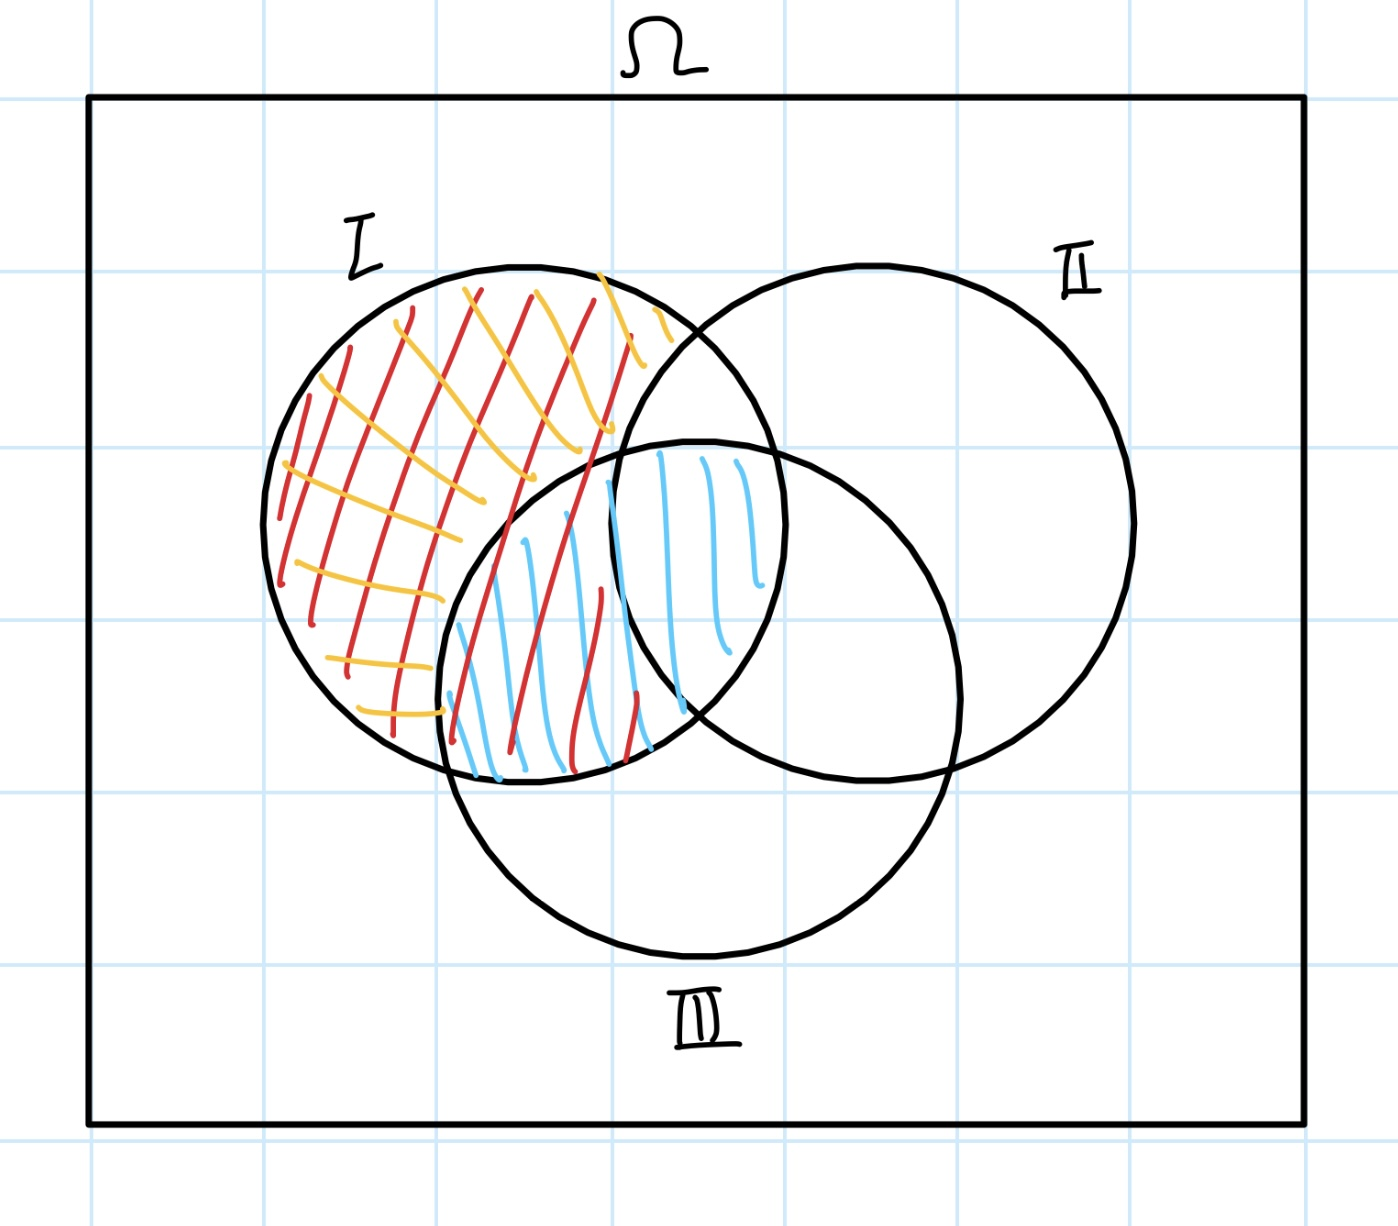
\includegraphics[width=60mm]{IMG_0702.jpg}
            \caption{Veen Diagram for Corresponding Statement}
        \end{center}
    \end{figure}

    Let $I, II, III$ denote the events of winning district I, II, III respectively (which represent the three circles in the Venn Diagram respectively). 
    
    Then, the event of winning I and III is represented by $I \cap III$, which is represented through the blue region in the Venn Diagram. Which, based on the given condition $\PP(I\cap III)=0.55$ (which corresponds to the area of the blue region).

    Similarly, the event of losing II and winning I is represented by $II^c \cap I$,which is represented through the red region in the Venn Diagram; and, the event of losing II,III and winning I is represented through $II^c \cap III^c\cap I$, and it's represented through the yellow region in the Venn Diagram. Thn, the conditions provided in the problem state that $\PP(II^c\cap I)=0.34$ (corresponds to the area of the red region), and $\PP(II^c\cap III^c\cap I)=0.15$ (corresponds to the area of the yellow region).

    \hfil

    Now, if consider the event of winning all three districts, it's represented by $I\cap II\cap III$. Which, we know $I\cap II\cap III = (I\cap III)\setminus ((I\cap III)\cap (II^c \cap I))$ (or the blue region excluding its intersection with the red region), hence, we get:
    \begin{align}
        \PP(I\cap II\cap III) = \PP(I\cap III)-\PP((I\cap III)\cap (II^c\cap I)) = 0.55 -\PP((I\cap III)\cap (II^c\cap I))
    \end{align}
    Also, we know $(I\cap III)\cap (II^c\cap I) = (II^c\cap I)\setminus (II^c\cap III^c\cap I)$ (or the red region excluding the intersection with yellow region, based on the Venn Diagram), hence with $(II^c\cap III^c\cap I)\subseteq (II^c\cap I)$, we get:
    \begin{align}
        \PP((I\cap III)\cap (II^c\cap I)) = \PP(II^c\cap I)-\PP(II^c\cap III^c\cap I) = 0.34 - 0.15 = 0.19
    \end{align}
    Combining the two equations, we get:
    \begin{align}
        \PP(I\cap II\cap III)=0.55 - 0.19 = 0.36
    \end{align}
\end{proof}

\newpage

\begin{ques}\label{q9}
    Chapter 1.4 \# 28

    Let $A_1,A_2,A_3,...$ be a sequence of events of a sample space. Prove that 
    $$\PP\left(\bigcup_{n=1}^\infty A_n\right)\leq \sum_{n=1}^\infty \PP(A_n)$$
    This is called \textbf{Boole's Inequality}.
\end{ques}

\begin{proof}
    If we assume that countable union of events $\bigcup_{n=1}^\infty A_n$ is an event, then define a sequence $(x_k)_{k\in\NN}\subset [0,1]$ by $x_k := \PP\left(\bigcup_{n=1}^k A_n\right)$. Then, for all $k\in\NN$, since $\bigcup_{n=1}^k A_n \subseteq \bigcup_{n=1}^{(k+1)}A_n$, it follows that $x_k = \PP\left(\bigcup_{n=1}^k A_n\right)\leq \PP\left(\bigcup_{n=1}^{(k+1)} A_n\right)=x_{k+1}$, hence $(x_k)_{k\in\NN}$ is a monotonically nondecreasing sequence bounded above by $1$, hence its limit exists and is finite. Then, given that the limit of probability function exists for increasing (or decreasing) inclusion chain of events, we get:
    \begin{align}
        \lim_{k\rightarrow \infty}x_k = \lim_{k\rightarrow\infty}\PP\left(\bigcup_{n=1}^k A_n\right) = \PP\left(\bigcup_{n=1}^\infty A_n\right)
    \end{align}
    Which, notice that for each $k\in\NN$, the following inequality holds:
    \begin{align}
        x_k = \PP\left(\bigcup_{n=1}^k A_n\right) \leq \sum_{n=1}^k \PP(A_n)
    \end{align}
    Hence, by taking the limit on both sides, we deduce the following:
    \begin{align}
        \PP\left(\bigcup_{n=1}^\infty A_n\right) = \lim_{k\rightarrow\infty}x_k \leq \lim_{k\rightarrow\infty}\sum_{n=1}^k\PP(A_n) = \sum_{n=1}^\infty\PP(A_n)
    \end{align}
\end{proof}

\hfil

\begin{ques}\label{q10}
    Chapter 1.7 \# 8

    Let $A_1,A_2,...,A_n$ be $n$ events. Show that if 
    $$\PP(A_1)=\PP(A_2)=...=\PP(A_n)=1$$
    then $\PP(A_1\cap A_2 \cap ... \cap A_n)=1$.
\end{ques}

\begin{proof}
    If given that $\PP(A_i)=1$ for all index $i=1,...,n$, then $\PP(A_i^c) = 0$ for all corresponding index $i$. Then, if consider $\left(\bigcap_{i=1}^n A_i\right)^c = \bigcup_{i=1}^n A_i^c$, then one can apply the following inequality:
    \begin{align}
        \PP\left(\left(\bigcap_{i=1}^n A_i\right)^c\right)=\PP\left(\bigcup_{i=1}^n A_i^c\right)\leq \sum_{i=1}^n \PP(A_i^c) = 0
    \end{align}
    Hence, as a result $\PP\left(\bigcap_{i=1}^n A_i\right)=1-\PP\left(\left(\bigcap_{i=1}^n A_i\right)^c\right)=1-0=1$.
\end{proof}

\end{document}